% ワークシート問3：y = a^x のグラフ（2点 (0,1)・(2,9) を通る。a = 3）（CC BY-SA 4.0）
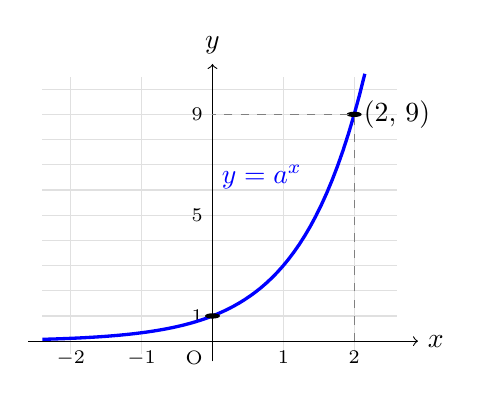
\begin{tikzpicture}[xscale=0.9,yscale=0.32]
  \draw[step=1,black!12,yscale=1] (-2.4,-0.5) grid (2.6,10.5);
  \draw[->] (-2.6,0) -- (2.9,0) node[right] {$x$};
  \draw[->] (0,-0.8) -- (0,11) node[above] {$y$};
  \foreach \t in {-2,-1,1,2} \node[below,font=\scriptsize] at (\t,0) {$\t$};
  \node[below left,font=\scriptsize] at (0,0) {O};
  \foreach \t in {1,5,9} \node[left,font=\scriptsize] at (0,\t) {$\t$};
  \draw[very thick,blue,domain=-2.4:2.15,samples=60] plot (\x,{3^\x});
  \fill (0,1) circle (3pt);
  \fill (2,9) circle (3pt) node[right] {$(2,\,9)$};
  \draw[dashed,black!50] (2,0) -- (2,9) -- (0,9);
  \node[blue,left] at (1.4,6.5) {$y = a^x$};
\end{tikzpicture}
